% Skip over this boring header down a bit
%%%%%%%%%%%%%%%%%%%%%%%%%%%%%%%%%%%%%%%%%%%%%%%%
\documentclass[usenames,dvipsnames,10pt,aspectratio=169]{beamer} 
% Add option 'aspectratio=169' for 16:9 widescreen 
% Add option  'handout' to ignore animations
% If you have a smaller amount of text, feel free to also try '11pt'! / Jesper

\usepackage[utf8]{inputenc}
\usepackage{verbatim}
\usepackage{minted}
\usemintedstyle{monokai}
\usepackage{graphicx}
\usepackage{wrapfig}
\usepackage[document]{ragged2e}
\usetheme{umu}

\usepackage{hyperref}
\hypersetup{
    colorlinks=true,
    linkcolor=ucuyellow,
    filecolor=ucuyellow,      
    urlcolor=ucuyellow,
}
\urlstyle{same}

\usepackage[shortlabels]{enumitem}

%%% Bibliography
\usepackage[style=authoryear,backend=biber]{biblatex}
\addbibresource{bibliography.bib}

\DeclareNameAlias{author}{given-family}

%%% Suppress biblatex annoying warning
\usepackage{silence}
\WarningFilter{biblatex}{Patching footnotes failed}

%%% Some useful commands
% pdf-friendly newline in links
\newcommand{\pdfnewline}{\texorpdfstring{\newline}{ }} 
% Fill the vertical space in a slide (to put text at the bottom)
\newcommand{\framefill}{\vskip0pt plus 1filll}

%%% Enter additional packages below 
\renewcommand{\proofname}{\sffamily{Proof}}

%%%%%%%%%%%%%%%%%%%%%%%%%%%%%%%%%%%%%%%%%%%%%%%%%%%%%%%%%%%%%%%%%%%%%%%%%%%%%%%%%%%%%
\title[Rust \#4]{Rust \#4: Smart pointers,\\ \vspace{0.1cm}Concurrency and Async}
\author[Sultanov Andriy]{Sultanov Andriy}
\institute{APPS@UCU}

\begin{document}

\begin{frame}
\titlepage
\end{frame}

\begin{frame}{\contentsname}
\tableofcontents
\end{frame}

\framepic{graphics/7.jpg}{
 \textcolor{ucuwhite}{Smart pointers}
 \vskip 0.5cm
 }

\section{Smart pointers}

\begin{frame}{Smart pointers}
	\framesubtitle{General}
\large	
Rust standard library has a few useful smart pointers, which\\
modify the possibilities of operating with the value they hold:\\
\vspace{0.4cm}
\begin{itemize}[label=$\bullet$]
	\item \textcolor{ucuyellow}{Box<T>}
	\item \textcolor{ucuyellow}{Rc<T>}
	\item \textcolor{ucuyellow}{Cell<T>}
	\item \textcolor{ucuyellow}{RefCell<T>}
\end{itemize}
\end{frame}

\begin{frame}{Smart pointers}
	\framesubtitle{Deref trait}
	\large
Implementing \textcolor{ucuyellow}{Deref} allows Rust to treat smart\\
pointers as references to the values they hold.\\
\vspace{0.4cm}
You can dereference types impementing \textcolor{ucuyellow}{Deref}\\
explicitly using the \textcolor{ucuyellow}{*} operator, or you can omit\\
the dereferencing and let Rust implicitly coerce\\
your type to the type you need.\\
\vspace{0.4cm}
Thus, when calling a method on a type that\\
implements \textcolor{ucuyellow}{Deref} and does not implement the\\
method, Rust will recursively dereference this\\
type until it finds the appropriate method.
\end{frame}

\begin{frame}{Smart pointers}
	\framesubtitle{Deref trait}
	\large
	So, let's say we want to have this kind of OOP\\
	behavior in Rust:
	\vspace{0.4cm}
	\inputminted[fontsize=\normalsize]{java}{code/deref1.rs}
\end{frame}

\begin{frame}{Smart pointers}
	\framesubtitle{Deref trait}
	\large
	We can model it like this:
	\vspace{0.1cm}
	\inputminted[fontsize=\footnotesize]{rust}{code/deref2.rs}
	\vspace{0.4cm}
\end{frame}

\begin{frame}{Smart pointers}
	\framesubtitle{Deref trait}
	\large
	And then easily use it:
	\vspace{0.4cm}
	\inputminted[fontsize=\large]{rust}{code/deref3.rs}
	\vspace{0.4cm}
	This allows you to easily operate with Rust's smart pointers.
\end{frame}

\begin{frame}{Smart pointers}
	\framesubtitle{Deref trait}
	\large
	Rust will coerce types according to these rules:
	
\begin{itemize}[label=$\bullet$]
	\item From \textcolor{ucuyellow}{\&T} to 
		\textcolor{ucuyellow}{\&U} when 
		\textcolor{ucuyellow}{T: Deref<Target=U>}
	\item From \textcolor{ucuyellow}{\&mut T} to
		\textcolor{ucuyellow}{\&mut U} when 
		\textcolor{ucuyellow}{T: DerefMut<Target=U>}
	\item From \textcolor{ucuyellow}{\&mut T} to
		\textcolor{ucuyellow}{\&U} when
		\textcolor{ucuyellow}{T: Deref<Target=U>}
\end{itemize}
\end{frame}

\begin{frame}{Box<T>}
	\large
	Boxes are Rust's way to store data on the heap.\\
	\vspace{0.4cm}
	They are useful when you want to handle values whose\\
	sizes can not be known at compile time as if their size\\
	was known. This works since the size of the pointer to\\
	the heap that the Box keeps on the stack is known.\\
\end{frame}

\begin{frame}{Box<T>}
	\large
	An example of moving a type that is typically stored\\
	on the stack onto the heap:
	\vspace{0.4cm}
	\inputminted[fontsize=\large]{rust}{code/box1.rs}
	\vspace{0.4cm}
	The value is going to be deallocated once it goes out\\
	scope, calling Box's \textcolor{ucuyellow}{drop} implementation.\\
\end{frame}

\begin{frame}{Box<T>}
	\large
	We could have just as well explicitly dereferenced the Box:
	\vspace{0.4cm}
	\inputminted[fontsize=\large]{rust}{code/box2.rs}
\end{frame}


\begin{frame}{Box<T>}
	\large
	If you want to create an unsized data structure, for\\
	example a recursive cons list, you can just use Box:
	\vspace{0.4cm}
	\inputminted[fontsize=\normalsize]{rust}{code/box3.rs}
	\vspace{0.2cm}
	What will end up being stored is an \textcolor{ucuyellow}{i32} and a\\
	pointer \textcolor{ucuyellow}{usize} to another List on the heap.
\end{frame}

\begin{frame}{Rc<T>}
	\large
	While Rust's ownership system is pretty strict, there\\
	are some ways to have multiple ownership. \textcolor{ucuyellow}{Rc<T>} is\\
	a reference counter that keeps track of the number\\
	of pointers to a certain value, and drops it once\\
	nobody uses it anymore.
\end{frame}

\begin{frame}{Rc<T>}
	\large
	\textcolor{ucuyellow}{Rc<T>} does not allow mutability, and basically changes\\
	the ownership system so that the control over the lifetime\\
	of the value is done during runtime, not compile time.\\
\end{frame}


\begin{frame}{Rc<T>}
	\inputminted[fontsize=\normalsize]{rust}{code/rc1.rs}
	\vspace{0.4cm}
\end{frame}

\begin{frame}{Others}
	\large
	Rust also provides several other standard smart pointers,\\
	like \textcolor{ucuyellow}{Cell<T>} and \textcolor{ucuyellow}{RefCell<T>}, which
	allow mutating the\\
	immutable value in various cases.\\
	\vspace{0.4cm}
	We are not going to cover them in these lectures, but\\
	it's important to understand how all of these smart\\
	pointers work under the hood, and the way they allow\\
	us to operate with the values they hold - through \textcolor{ucuyellow}{Deref}.
\end{frame}

\framepic{graphics/7.jpg}{
 \textcolor{ucuwhite}{Concurrency}
 \vskip 0.5cm
 }

\section{Concurrency}

\begin{frame}{Concurrency in general}
	\large
	We've talked about how computers work in general before,\\
	but we've always implicitly assumed that they only run one\\
	thing at a time - that is, we've talked about a single-core CPU.\\
	\vspace{0.3cm}
	How are user programs represented for that CPU? Through\\
	the abstraction of a process - an instance of a program in\\
	execution. It might be better to think of the process as the\\
	collection of data structures that fully describes the state\\
	of the execution of a certain program.\\
\end{frame}

\begin{frame}{Concurrency in general}
	\large
\begin{wrapfigure}{r}{0.5\textwidth}
\centering
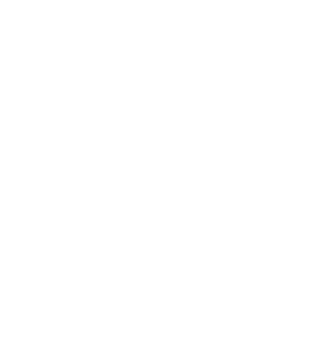
\includegraphics[width=0.7\linewidth]{graphics/process1.png}
\end{wrapfigure}
	Thus, a process can roughly be\\
	represented as this, a\\
	collection of data structures\\
	that describe it,
	and a single thread of execution that is\\
	actually scheduled for\\
	execution and handles\\
	the state of the program.
\vspace{2.8cm}
\end{frame}

\large
\begin{frame}{Concurrency in general}
\begin{wrapfigure}{r}{0.5\textwidth}
\centering
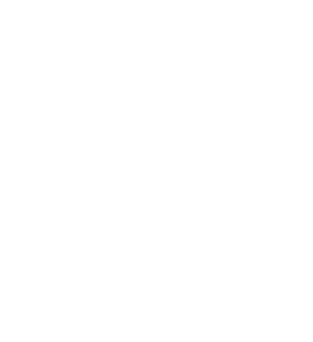
\includegraphics[width=0.7\linewidth]{graphics/process2.png}
\end{wrapfigure}
	One process can contain\\
	multiple threads of\\
	execution though, which\\
	are going to have the same shared memory and code
	through the process, but are going to be running different code
	simultaneously.
	\vspace{2.8cm}
\end{frame}

\begin{frame}{Concurrency in general}
	\large
	The task of scheduling and prioritizing these threads\\
	falls on the operating system, which allows creating\\
	these structures in the first place, and maintains\\
	a list of them, periodically switching the CPUs\\
	to run this or that thread.\\
	\vspace{0.3cm}
	We are not going to talk about multithreading from\\
	the OS perspective, but it's important to understand\\
	what happens with our CPU once we have multiple cores\\
	and are able to execute several threads at a time.
\end{frame}

\begin{frame}{Concurrency in general}
\begin{wrapfigure}{r}{0.5\textwidth}
\centering
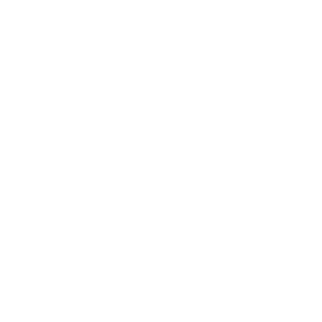
\includegraphics[width=0.7\linewidth]{graphics/process3.png}
\end{wrapfigure}
	
\large
The operating system and the CPU handle all of
the minor details of the process of scheduling
and actually executing the threads on several
cores, we are just going to assume that all of this
works nicely (it almost always does)!
\vspace{2.8cm}
\end{frame}

\begin{frame}{Concurrency in general}
\begin{wrapfigure}{r}{0.5\textwidth}
\centering
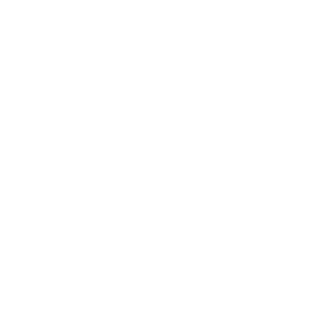
\includegraphics[width=0.7\linewidth]{graphics/process4.png}
\end{wrapfigure}
	
\large
The operating system and the CPU handle all of
the minor details of the process of scheduling
and actually executing the threads on several
cores, we are just going to assume that all of this
works nicely (it almost always does)!
\vspace{2.8cm}
\end{frame}

\begin{frame}{Synchronization}
	\large
	We've already talked about how a safe system would look like,
	where nobody will violate the memory safety of others:
	\vspace{0.4cm}
	\begin{itemize}[label=$\bullet$]
		\item There can be many readers with no writers at the same time
		\item There can be only one writer with no readers at the same time
		\item Values can be used only as long as they still exist
	\end{itemize}
	\vspace{0.4cm}
	We've seen how Rust ensures all of these rules are\\
	satisfied in a single-thread scenario, but what if\\
	there are several threads running at the same time?\\
	How do we make sure they don't write into each other's\\
	memory?
\end{frame}

\begin{frame}{Concurrency}
	\large
	\textcolor{ucured}{TODO: Talk about Arc, Mutex,
	mspc, and the way Rust's system prevents data races at compile
time.}
\end{frame}

\framepic{graphics/7.jpg}{
 \textcolor{ucuwhite}{Looking back}
 \vskip 0.5cm
 }

\section{Looking back}

\begin{frame}{Looking back}
	\large
	Over the course of four weeks we've covered\\
	some general topics, which I hope you will\\
	be able to apply everywhere, not only in Rust:\\
	\vspace{0.1cm}
\begin{itemize}[label=$\bullet$]
	\item Machine memory model
	\item Safe mutability rules
	\item Safe ownership and lifetime rules
	\item Multithreading
\end{itemize}
	
\end{frame}

\begin{frame}{Looking back}
	\large
	And we've also looked at quite a lot of\\
	Rust-specific stuff:
	\vspace{0.1cm}
\begin{itemize}[label=$\bullet$]
	\item Rust's ownership/lifetime/mutability system
	\item Cargo ecosystem
	\item Algebraic types and error handling
	\item Declarative macros
	\item Traits
	\item Iterators and closures
	\item Multithreading primitives
\end{itemize}
\end{frame}
\framepic{graphics/7.jpg}{
 \textcolor{ucuwhite}{And ahead...}
 \vskip 0.5cm
 }

\section{And ahead...}

\begin{frame}{Looking ahead}
	\large
There is quite a lot of stuff in Rust that we haven't\\
covered. If you want to dive deeper yourself, here is\\
a short list of some of the most important things you\\
can look into:
\vspace{0.2cm}
\begin{itemize}[label=$\bullet$]
	\item Async Rust
	\item Procedural macros
	\item Testing
	\item FFI and bindings
\end{itemize}
\vspace{0.2cm}
And many more...
\end{frame}

\begin{frame}{Looking ahead}
\Large
But, most importantly, practice makes perfect!\\

\vspace{0.4cm}
I hope that this short tour of Rust has shown\\
you the possibilities of modern languages and\\
ecosystems, and taught you a few important\\
things in general!
\end{frame}

\framepic{graphics/7.jpg}{
	\textcolor{ucuwhite}{Thank you!}
 \vskip 0.5cm
 }

\end{document}
